\documentclass[conference]{IEEEtran}
\IEEEoverridecommandlockouts
% The preceding line is only needed to identify funding in the first footnote. If that is unneeded, please comment it out.
\usepackage{cite}
\usepackage{amsmath,amssymb,amsfonts}
\usepackage{algorithmic}
\usepackage{graphicx}
\usepackage{textcomp}
\usepackage{xcolor}
\usepackage{multirow,array}
\def\BibTeX{{\rm B\kern-.05em{\sc i\kern-.025em b}\kern-.08em
    T\kern-.1667em\lower.7ex\hbox{E}\kern-.125emX}}

\colorlet{dark-cyan}{cyan!75!black}
\newcommand\katja[1]{{\color{dark-cyan}Katja: #1}}

\newcommand\TODO[1]{{\color{red}TODO: #1}}
\newcommand\MAYBE[1]{{\color{blue} #1}}

\begin{document}

\title{Win or Learn Fast Proximal Policy Optimisation (WoLF-PPO)}

\author{\IEEEauthorblockN{1\textsuperscript{st} Given Name Surname}
\IEEEauthorblockA{\textit{dept. name of organization (of Aff.)} \\
\textit{name of organization (of Aff.)}\\
City, Country \\
email address}
\and
\IEEEauthorblockN{2\textsuperscript{nd} Given Name Surname}
\IEEEauthorblockA{\textit{dept. name of organization (of Aff.)} \\
\textit{name of organization (of Aff.)}\\
City, Country \\
email address}
\and
\IEEEauthorblockN{3\textsuperscript{rd} Given Name Surname}
\IEEEauthorblockA{\textit{dept. name of organization (of Aff.)} \\
\textit{name of organization (of Aff.)}\\
City, Country \\
email address}
}

\maketitle

\begin{abstract}
% draft 0
%    We consider learning strategies in fully competitive zero-sum games. There have been two main properties identified as desirable for agents that learn in  such settings. This includes being convergent in self play, where the agent learns a Nash Equilibrium Strategy (NES) and minimizing regret when dealing with opponent agents that are playing a stationary policy. One approach for dealing with these problems is Win or Learn Fast (WoLF), this approach has been shown to converge to NES in self play, as well as playing best response when playing against stationary opponents. In this paper we look to combine the recent advancements in Deep Reinforcement Learning with Win or Learn Fast. In particular - we focus on a policy gradient algorithm, PPO, which has shown excellent empirical performance in multi-agent scenarios (self-play). We present a systematic empirical investigation into whether WoLF can be effectively adapted to this state of the art algorithm, and whether the characteristics of WoLF continue to hold. We demonstrate that WoLF is able to improve the performance of PPO in multiple environments and give insight into environment properties that help PPO learn a strategy close to the NES.

% draft 1
    In order to solve many problems agents are required to compete within an environment shared by many other agents. This problem is tackled by multiagent reinforcment leanring (MARL). Treating multiagent problems as simply non-stationary environments has been shown to produce sub optimal performance. One solution to MARL is to learn a Nash Equilibrium that guarantees a known minimum payoff when playing against other rational agents. We focus on one approach for learning Nash equilibria, Win or Learn Fast (WoLF). WoLF has been shown to converge towards Nash equilibria in a variety of matrix-games and grid based games. We present a systematic empirical investigation into whether WoLF can be effectively adapted to Deep RL, and the characteristics of using WoLF with function approximation. We demonstrate that WoLF is able to improve the performance of Proximal Policy Optimisation (PPO) in multiple environments and give insight into environment properties that help PPO learn strategies close to the Nash Equilibrium.
\end{abstract}

\begin{IEEEkeywords}
\TODO{keywords}
\end{IEEEkeywords}
\section{Introduction}

% draft 0
%In multi-agent games the optimal strategy is linked to the strategy of the other players within the environment. This results in different optimal strategies depending on the opponent. One way of tackling this problem is to consider the Nash Equilibrium of a game. The Nash equilibrium is a strategy that if all the player are playing in a Nash equilibrium no one player can increase their payoff by changing their strategy. This means there exists a stationary policy that is minimally exploitable against agents that are trying to maximise their own reward. This gives us a target policy to learn that can be frozen and has a known minimum payoff.
%
%There are problems when trying to learn in multi-agent systems. If we are training against a learning opponent then we are constantly trying to hit a moving target as the opponents policy updates over time. This results in traditional reinforcment learning agents cycling through policies around the Nash equilibrium, meaning if we freeze the policy at any point it would be a sub optimal solution when an agent is trained against that stationary policy. Some agents covered in this paper will pre-compute the Nash equilibrium ahead of training in order to use that policy if it detects that the opponent is learning, this will work well for simple environments were it is relatively easy to compute the Nash equilibrium but will not scale to larger multi-agent environments.
%
%Previous work in this area has highlighted two properties that would be desirable for agents learning in multi-agent environments. The first property is rationality, this property states that the agent should learn a best response to any policy that it converges to. The second property is convergence this states that the agent must converge to a stationary policy, for some class of learning algorithms. If an agent conforms to both of these properties then it will converge to a Nash equilibrium.
%
%In this paper we look to extend WoLF to Deep Reinforcement learning. We do this by comparing the performance of standard PPO, a state of the art Deep RL algorithm, to a new approach WoLF-PPO. We evaluate them in traditional game theory matrix-games, we also test the performance on variations of these games that shift the Nash equilibrium.
%
%We show that WoLF in Deep Reinforcment learning dies have a positive effect, we also demonstrate that in some multi-agent environments PPO achieves good performance. This is specifically in environments were the Nash policy is the Max-Entropy policy.

% draft 1
In multiagent environments the learning problem is non-stationary due to the fact that the other agents polices are changing over time. Traditional Reinforcment Learning (RL) techniques have garuntees that rely on the probelm domain being a Markov Decision Process (MDP), given the multi-agent environment is non-stationary this does not hold and the guarantees are lost. There has however been work in MARL that aims to tackle this problem, the work we focus on is Win or Learn Fast (WoLF) that is a technique that uses variable learning rates to give guarantees of converging to a Nash Equilibrium Strategy (NES). Learning a NES is very desirable as it allows us to learn a fixed policy that has a known lower bound payoff when dealing with rational agents.

In this paper we perform an initial study into the applicability of extending WoLF into Deep RL. We present an extension to proximal policy optimisation WoLF-PPO that is targeted at learning NES within mulitagent environments. We compare WoLF-PPO to PPO in a variety of traditional game theory matrix-games and demonstrated that WoLF has a positive effect when trying to learn NES using Deep RL.

\section{Background}

\subsection{Game Frameworks}

\subsubsection{Markov Decision Process} is the framework that is used for dealing with reinforcement
learning in the single agent environment. MDP can be represented by the tuple 
$(\mathcal{S}, \mathcal{A}, \mathcal{T}, \mathcal{R})$ were $S$ is the set of possible
states, $A$ is the set of possible actions, $T$ is a transition function of the form 
$\mathcal{S}\times\mathcal{A}\times\mathcal{S}\rightarrow [0,1]$ that gives a probability
distribution over next states after a given action is performed in a given state. Finally
$R$ represents a reward function of the form $\mathcal{S}\times\mathcal{A}\rightarrow \mathbb{R}$
that returns a reward when a given action is performed on a given state. This framework presents a problem that can be solved by maximising the discounted
future reward with a given discount factor denoted by $\gamma$. All MDPs can be solved
with a stationary deterministic policy, this results in the majority of single agent
RL work focusing on agents that solve this type of problem without much consideration
of how they may perform in a multiagent environment where a deterministic strategy may
not be optimal.

\subsubsection{Matrix Games}

A framework that does deal with multiple agents are matrix games. These games
can be represented by the following tuple $(n, \mathcal{A}_{1...n}, \mathcal{R}_{1...n})$
where $n$ represents the number of agents, $\mathcal{A}_{i}$ represents the actions
available to agent $i$ with $A$ representing the joint action between all agents and 
$\mathcal{R}_{i}$ represents the reward function for agent $i$. It is the reward 
function that gives this framework its name as it can easily be represented as 
$n$ set of matrices. Matrix games have a couple of different forms as either zero-sum games or general-sum
games. Zero-sum games are strictly competitive, were if one of the agents receives a
positive reward then the opposing agent receives a negative reward, this can sum to 
either zero or some other constant. General-sum games do not have this constraint and
can even have reward matrices that are identical across agents, resulting in strictly
cooperative games. When considering what solved means for this framework two properties emerge, they are
the Best Response strategy and the Nash Equilibrium. The best response strategy is the optimal strategy against the joint actions of all the
other agents. In the case of playing against a set of stationary opponents there will 
exist a deterministic best response strategy. Nash equilibrium takes this one step further and states that all agents should be playing
a best response against the joint actions of all its respective opponents. This produces
a dynamic where an agent playing the Nash equilibrium can not do better by changing strategy
whilst the other agents are also playing a Nash equilibrium. This does not mean that the
Nash equilibrium is an optimal strategy against all agents however it does provide 
stability by preventing the agent from being exploited by another strategy. Nash equilibrium
have also been proven to exist in all zero-sum games (contain a unique Nash equilibrium) and
all general sum games, making it a very desirable strategy to be able to learn.

\subsubsection{Stochastic Games} is a frame work that combines the Markov Decision Process (MDP) framework and the 
Matrix games framework. It can be seen as a MDP with with multiple agents producing 
a joint action that is used for the transition function and agents reward function. Stochastic games can be seen as the fol owing tuple $(n, \mathcal{S}, \mathcal{A}_{1...n}, 
\mathcal{T}, \mathcal{R}_{1...n})$. This is with $n$ representing the number of agents 
in the game, $\mathcal{S}$ being the set of possible states, $\mathcal{A}_{i}$ being the 
set of actions available to agent $i$, $\mathcal{A}$ represents the set of joint actions, 
$\mathcal{T}$ is a transition function in the form of 
$\mathcal{S}\times\mathcal{A}\times\mathcal{S}\rightarrow [0, 1]$ giving a probability 
distribution over states that result from the joint action $\mathcal{A}$ being performed
on a given state, finally $\mathcal{R}_{i}$ is a reward function for agent $i$ in the form
$\mathcal{S}\times\mathcal{A}\rightarrow \mathbb{R}$. As stochastic games are built on MDP and matrix games both of these are subsets of
stochastic games. A stochastic game with all opposing agents having stationary policies
is identical to a MDP. If the Stochastic game only has one state then it is identical 
to a matrix game. Some of the properties from matrix games also transition over to stochastic games, 
this includes the notion of zero-sum games and general sum games. This also means
that Nash equilibrium strategies exist for stochastic games and this is the strategy
that the original WoLF work and our work is trying to learn.

\katja{best response? discuss other solution concepts if relevant}

\subsection{Properties of Multi-Agent systems}

Within multiagent literature two main properties have
been identified as desirable for any multiagent learning
system.

The first of these properties is rationality, this property requires
the agent to learn a best-response strategy against any agent that 
converges to a stationary policy. This is a relatively easy property to 
obtain, given that stochastic games with an opponent playing a stochastic 
policy can be framed as an MDP. So this means that any agent that can 
solve an MDP is rational by this definition.

The second property dictates that the agent will converge to a stationary policy given 
a stationary agent or a learning agent from a defined class. This class of learning
algorithms is usually defined as consisting of most "useful" algorithms (often restricted
to rational algorithms). In practise this results in most literature focusing on self 
play, however some work has been empirically shown to converge with a small subset of learning 
agents beyond self play. 

The reason that these two rules have been identified as desirable properties for mulitagent
systems to possess is how their relationship relates to the Nash equilibrium. This comes from 
the fact that if both agents are rational and both converge to a stationary policy then they
must have converged to a Nash equilibrium. This can logically be thought through, if both 
agents are guaranteed to play best response to a stationary policy then neither of the agents 
can individually change their strategy in order to increase their payoff. Given this the agents 
must have then converged to a Nash equilibrium.

\section{Related Work}

\subsection{WoLF}

Infinitesimal Gradient Ascent (IGA) has been proven in self play will either converge to a Nash equilibrium,
or the average payoffs over time will converge in the limit to a Nash Equilibrium. This provides an agent
that is both rational and convergent. However this is regarded as a week form of convergence as it may only
converge to the payoff of a Nash equilibrium in expectation. This work was then expanded on with variable
learning rates.

The introduction of a variable learning rate method, Win or Learn Fast (WoLF) looks to extend IGA into a
method that has a stronger notion of converging to a Nash equilibrium. This is done by introducing separate
learning rates for when the agent is winning and when it is losing. The agent is judged to be winning if their
current expected payoff is better than playing the Nash equilibrium. This change has the effect of the winning
agent learning slower and being more "cautious" about updating its strategy until the other agent has learned 
to counter the new strategy.

This approach does place some strict requirements on what knowledge is needed of the game. The method requires
the player's own payoff matrix to be known and the policy of the opponent agent. It would also need to know
the Nash Equilibrium in order to compute if the agent is currently winning or losing, this however can be 
computed from the known payoffs.

Although the proofs for this method do require knowing detailed information about the environment and opponent,
a practical algorithm has been presented. This method is based on PHC and uses a comparison of the current expected
payoff to the expected payoff of the current average policy. This provides a estimation of the equilibrium policy.

\subsection{Proximal Policy Optimisation}

Proximal Policy Optimisation (PPO) is a policy based gradient method for deep reinforcement learning. It is a current state of the art deep reinforcment leanring algorithm that has shown good results on atari games, mujoco control tasks and Dota 2. PPO is based on the ideas introduced with Trust Region Policy Optimisation (TRPO). It does this whilst trying trying to solve many problems with TRPO. TRPO is relatively complicated to implement when compared to other Deep RL methods, it is not compatible with architectures involving noise, making dropout unusable, similarly TRPO also doesn't allow for parameter sharing making shared layers between policy and value output impossible as well as training with auxiliary tasks.

PPO is able to improve these shortcomings of TRPO by introducting clipped probability ratios that can be used as a lower bound estimate of the policy performance. This means that PPO only requires first-order optimisation, making PPO easier to implement and support noisy architectures and parameter sharing. 

The objective function for PPO is shown in equation \ref{eq:ppo-objective}. 

\begin{equation}
    L_t^{CLIP+VF+S}(\theta) = \hat{\mathbb{E}}_t\big[L_t^{CLIP}(\theta)-c_1L_t^{VF}(\theta)+c_2S[\pi_{\theta}](S_t)\big]
    \label{eq:ppo-objective}
\end{equation}

$c_1$ and $c_2$ are coefficients. $S$ is the max entropy bonus and $L_t^{VF} = (V_{\theta}(s_t)-V_t^{targ})^2$. Here we can see that PPO has a term in its objective function that rewards higher entropy strategies $c_2S[\pi_{\theta}]$, this is to aid in expoloration at the begining of training in order to prevent the agent from learning a overly deterministic policy before exploring the state space. 

%\begin{equation}
%    L^{CPI}(\theta) = \hat{\mathbb{E}}_t\Bigg[\frac{\pi_{\theta}(a_t | s_t)}{\pi_{\theta_{old}}(a_t | s_t)}\hat{A}_t\Bigg] = \hat{\mathbb{E}}_t\bigg[r_t(\theta)\hat{A}_t\bigg]
%    \label{eq:trpo-objective}
%\end{equation}

\TODO{Explain clipping here? Not sure how much detail to go into, the fact it optimises max-etropy is the main takeaway about how PPO works for this paper? Should probably focus more detail here though and cut content else where}

PPO has shown state of the art results on control tasks and better sample comlexity on the Atari environments.

\subsection{Multi-Agent PPO}

There has been some previous work in applying PPO to multi-agent environments. In the work by ??et al, the main focus is the introduction of new competative multi-agent control tasks and how PPO performs in these environments, evaluating the effect of an "exploration" reward and opponent sampling. Many of their findings and observations are relevant to our work.The tasks introduced are two player fully competitive control tasks, including games that involve scoring goals or getting past the other player. These tasks also support two body types, Ant and humanoid. The environments are not directly related to our work as it would be difficult to evaluate the distance to the Nash equilibrium in these environments. They do however train PPO on these environments and make many useful observations. they asses the performance of PPO when using opponent sampling were old version of the opponent are sampled throughout training. They present that opponent sampling is a form of curriculum learning that is inherent in competative multi-agent environments.

They observe that without opponent sampling then one agent can begin to dominate the other and result in a strategy that has overfitted to the opponent policy. They manage to improve this by using opponent sampling over the course of training resulting in better final policies. They do note that uniform sampling is not always the best approach and demonstrate environments were weighting the sampling to more recent agents results in better performance.

they aslo observe that the agents final policies vary greatly from run to run with different random seeds. No attempt is made in thsi work to evaluate the distance from the Nash equilibrium. 

\section{Empirical Experiments}

For our empirical results we aimed to highlight the difference between PPO and WoLF-PPO, we have therefore used the same experimental setup and environments form the original WoLF paper, as these were also designed to highlight the advantages of WoLF. We also introduce some weighted variants the the environments to highlight the effect of the entropy term present in PPOs objective function.

\subsection{Network Setup}

Due to the simplicity of WoLF achieving convergence to Nash Equilibriums by varying the learning rate it is a relativly easy approach to apply to current Deep RL approaches. We chose to use PPO as the base agent as it has been shown to acheive good results in both single player environments and when training on large amounts of experience in complex multiagent environments \TODO{[AI5:ref]}. We vary our learning rate by a ratio of $\alpha$ where $\beta_{LOSE} = \alpha\beta_{WIN}$, for all experiments $\alpha = 4$. In order to make sure that adaptive learning rate optimisation such as ADAM or AdaGrad didn't have an effect on the variable learning rate we used standard Stochastic Gradient Descent (SGD) for all experiments. In order to evaluate if we are "winning" we also need to estimate if we are doing better than the Nash Equilibrium Strategy. In order to do this we average the payoff over training as this will provide an estimation of the payoff the agent would receive when playing the NES. This works well for the games presented but would need to be extended for extensive form games. In future wor kwe would like to present a method for learning an estimation of Nash using function approximation.

The network used for all experiments is a small fully connected feed forward neural network, two hidden layers of $20$ neurons, due to the simplicity of the experimental environments. We kept the network and experimental setup simple as we are attempting to establish the posibility of fruitful research in this area for the furture.

\subsection{Matching Pennies}

The first and simplest environment we used is Matching Pennies in both its original form with a uniform random Nash Equilibrium and a weighted form, were the Nash Equilibrium is shifted away from uniform random. The payoff matrices are shown in Tables \ref{tab:stock-mp} and \ref{tab:weighted-mp} respectivly. 
Matching pennies is a game were both players pick a side of a coin, either heads or tails, these choices are then reveled simultaneously with one player receiving a point if they match and the other receiving a point if they differ. This results in the Nash Equilibrium being uniform random, if you pick the side of the coin at random then you will win 50\% of the games irrespective of your opponents strategy.

\begin{table}
    \centering
    \setlength{\extrarowheight}{2pt}
    \begin{tabular}{*{4}{c|}}
      \multicolumn{2}{c}{} & \multicolumn{2}{c}{Player $2$}\\\cline{3-4}
      \multicolumn{1}{c}{} &  & $H$  & $T$ \\\cline{2-4}
      \multirow{2}*{Player $1$}  & $H$ & $(1,-1)$ & $(-1,1)$ \\\cline{2-4}
      & $T$ & $(-1,1)$ & $(1,-1)$ \\\cline{2-4}
    \end{tabular}
    \caption{Payoff matrix for standard Matching Pennies, with a Nash of uniform random.}
    \label{tab:stock-mp}
\end{table}

\begin{table}
    \centering
    \setlength{\extrarowheight}{2pt}
    \begin{tabular}{*{4}{c|}}
      \multicolumn{2}{c}{} & \multicolumn{2}{c}{Player $2$}\\\cline{3-4}
      \multicolumn{1}{c}{} &  & $H$  & $T$ \\\cline{2-4}
      \multirow{2}*{Player $1$}  & $H$ & $(2,-2)$ & $(-1,1)$ \\\cline{2-4}
      & $T$ & $(-1,1)$ & $(1,-1)$ \\\cline{2-4}
    \end{tabular}
    \caption{Payoff matrix for weighted Matching Pennies, with a Nash of $P(H)=0.2$.}
    \label{tab:weighted-mp}
\end{table}


\subsection{Rock Paper Scissors}

Moving up form matching Pennies we used Rock Paper Scissors as our next environment. This game consists of three possible actions that form a cyclic winning pattern, as shown in Table \ref{tab:rps}.

\begin{table}
    \centering
    \setlength{\extrarowheight}{2pt}
    \begin{tabular}{*{5}{c|}}
      \multicolumn{2}{c}{} & \multicolumn{2}{c}{Player $2$}\\\cline{3-5}
      \multicolumn{1}{c}{} &  & $R$  & $P$ & $S$ \\\cline{2-5}
      \multirow{2}*{Player $1$}  & $R$ & $(0,0)$ & $(-1,1)$ & $(1,-1)$ \\\cline{2-5}
      & $P$ & $(1,-1)$ & $(0,0)$ & $(-1,1)$ \\\cline{2-5}
      & $S$ & $(-1,1)$ & $(1,-1)$ & $(0,0)$ \\\cline{2-5}
    \end{tabular}
    \caption{Payoff matrix for standard Rock Paper Scissors, with a Nash of $P(Rock)=P(Papaer)=P(Scissors)=0.\dot{3}$.}
    \label{tab:rps}
\end{table}

This environment is of interest because many complex commercial games will have multi-agent scenarios that mimic Rock Paper Scissors [ref]. We again present the standard version of Rock Paper Scissors and a weighted variant to move the Nash Equilibrium away from uniform random. The payoff matrices for these versions can be found in Fig \TODO{put in fig}.

\begin{table}
    \centering
    \setlength{\extrarowheight}{2pt}
    \begin{tabular}{*{5}{c|}}
      \multicolumn{2}{c}{} & \multicolumn{2}{c}{Player $2$}\\\cline{3-5}
      \multicolumn{1}{c}{} &  & $R$  & $P$ & $S$ \\\cline{2-5}
      \multirow{2}*{Player $1$}  & $R$ & $(0,0)$ & $(-1,2)$ & $(1,-2)$ \\\cline{2-5}
      & $P$ & $(2,-1)$ & $(0,0)$ & $(-1,1)$ \\\cline{2-5}
      & $S$ & $(-2,1)$ & $(1,-1)$ & $(0,0)$ \\\cline{2-5}
    \end{tabular}
    \caption{Payoff matrix for weighted Rock Paper Scissors, with a Nash of $P(ROCK)=0.2$ and $P(PAPER)=0.4$.}
    \label{tab:weighted-rps}
\end{table}

\section{Results}

We now present our results on the two varients of the matrix games matching pennies and rock paper scissors. We focus on evaluating the distance of PPO and WoLF-PPO from the known Nash Equilibrium of these games. We also test the results of using large learning rates to identify any differences to robustness between the agents.

\subsection{Matching Pennies}

Starting with PPO and WoLF-PPO on the standard weighting of matching pennies we can see that both agents stay close to the Nash equilibrium as shown in Fig \ref{fig:mp-ppo-e2}. You can see that the variance for PPO is still within $0.05$ of the Nash equilibrium. In this setting we see that WoLF-PPO does indeed have lower variance than PPO but not by a large margin.

\begin{figure}
    \centering
    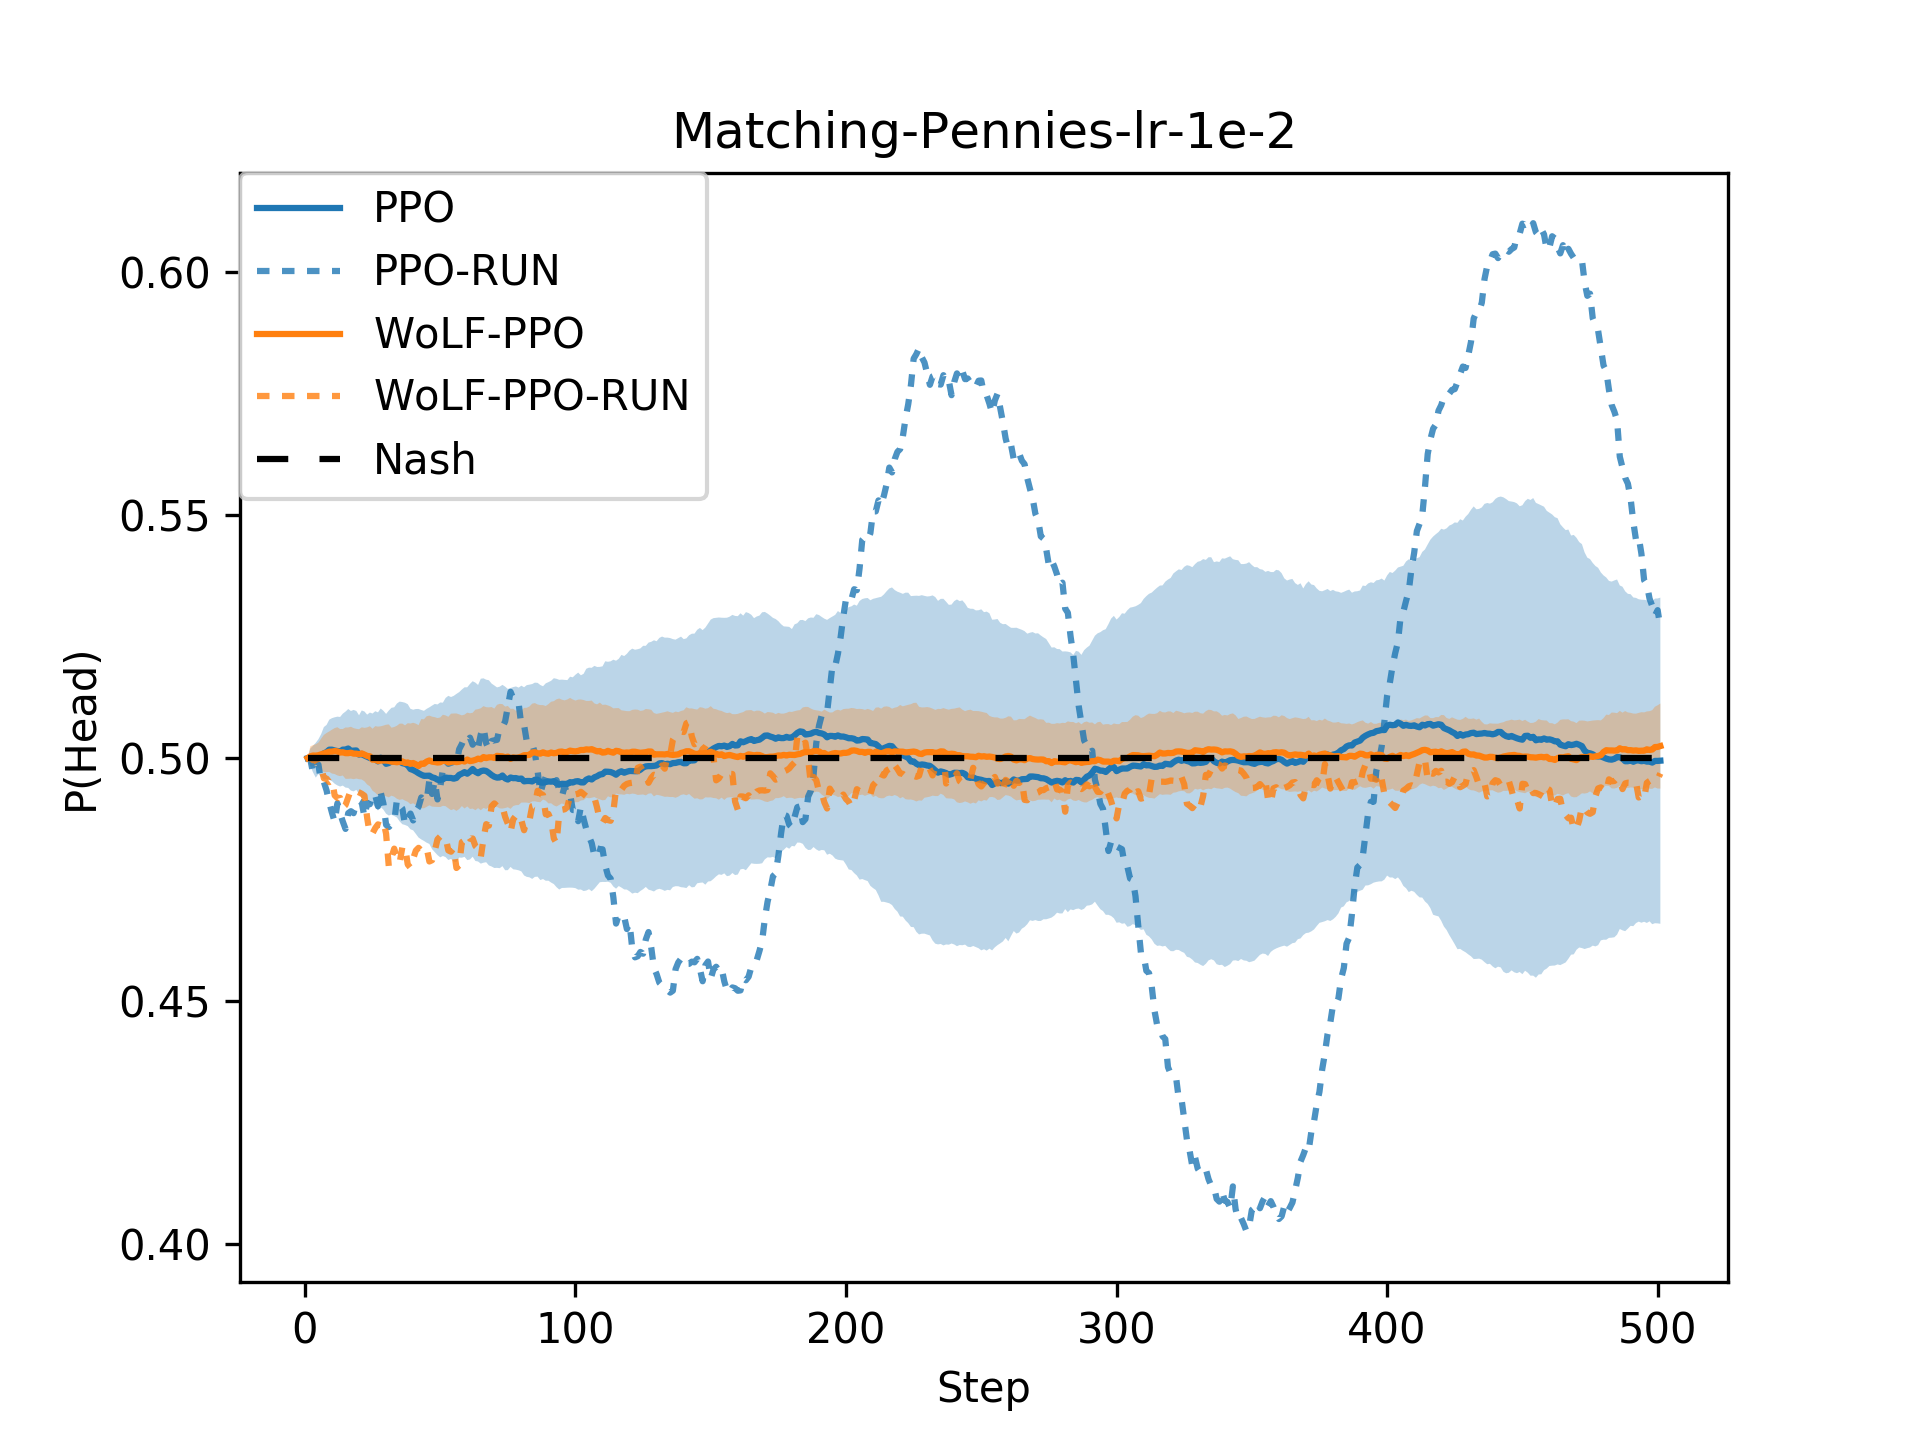
\includegraphics[width=20em]{Figures/matching-pennies-lr-1e-2.png}
    \caption{With a reasonable learning rate of 1e-2 for PPO both agents learn strategies close to the Nash equilibrium.}
    \label{fig:mp-ppo-e2}
\end{figure}

When the learning rate is increased by an order of magnitude as in Fig \ref{fig:mp-ppo-e1}, it is apparent that the variance away from the Nash equilibrium increases for both PPO and WoLF-PPO, however WoLF-PPO stays much closer to the Nash equilibrium. We believe that the relatively good performance of PPO in this environment is due to the maximizing of entropy in PPOs objective function. In games such as matching pennies the Nash equilibrium is to play uniform random and thus max entropy. That results in this version of matching pennies having its Nash equilibrium directly optimized in the objective function.

\begin{figure}
    \centering
    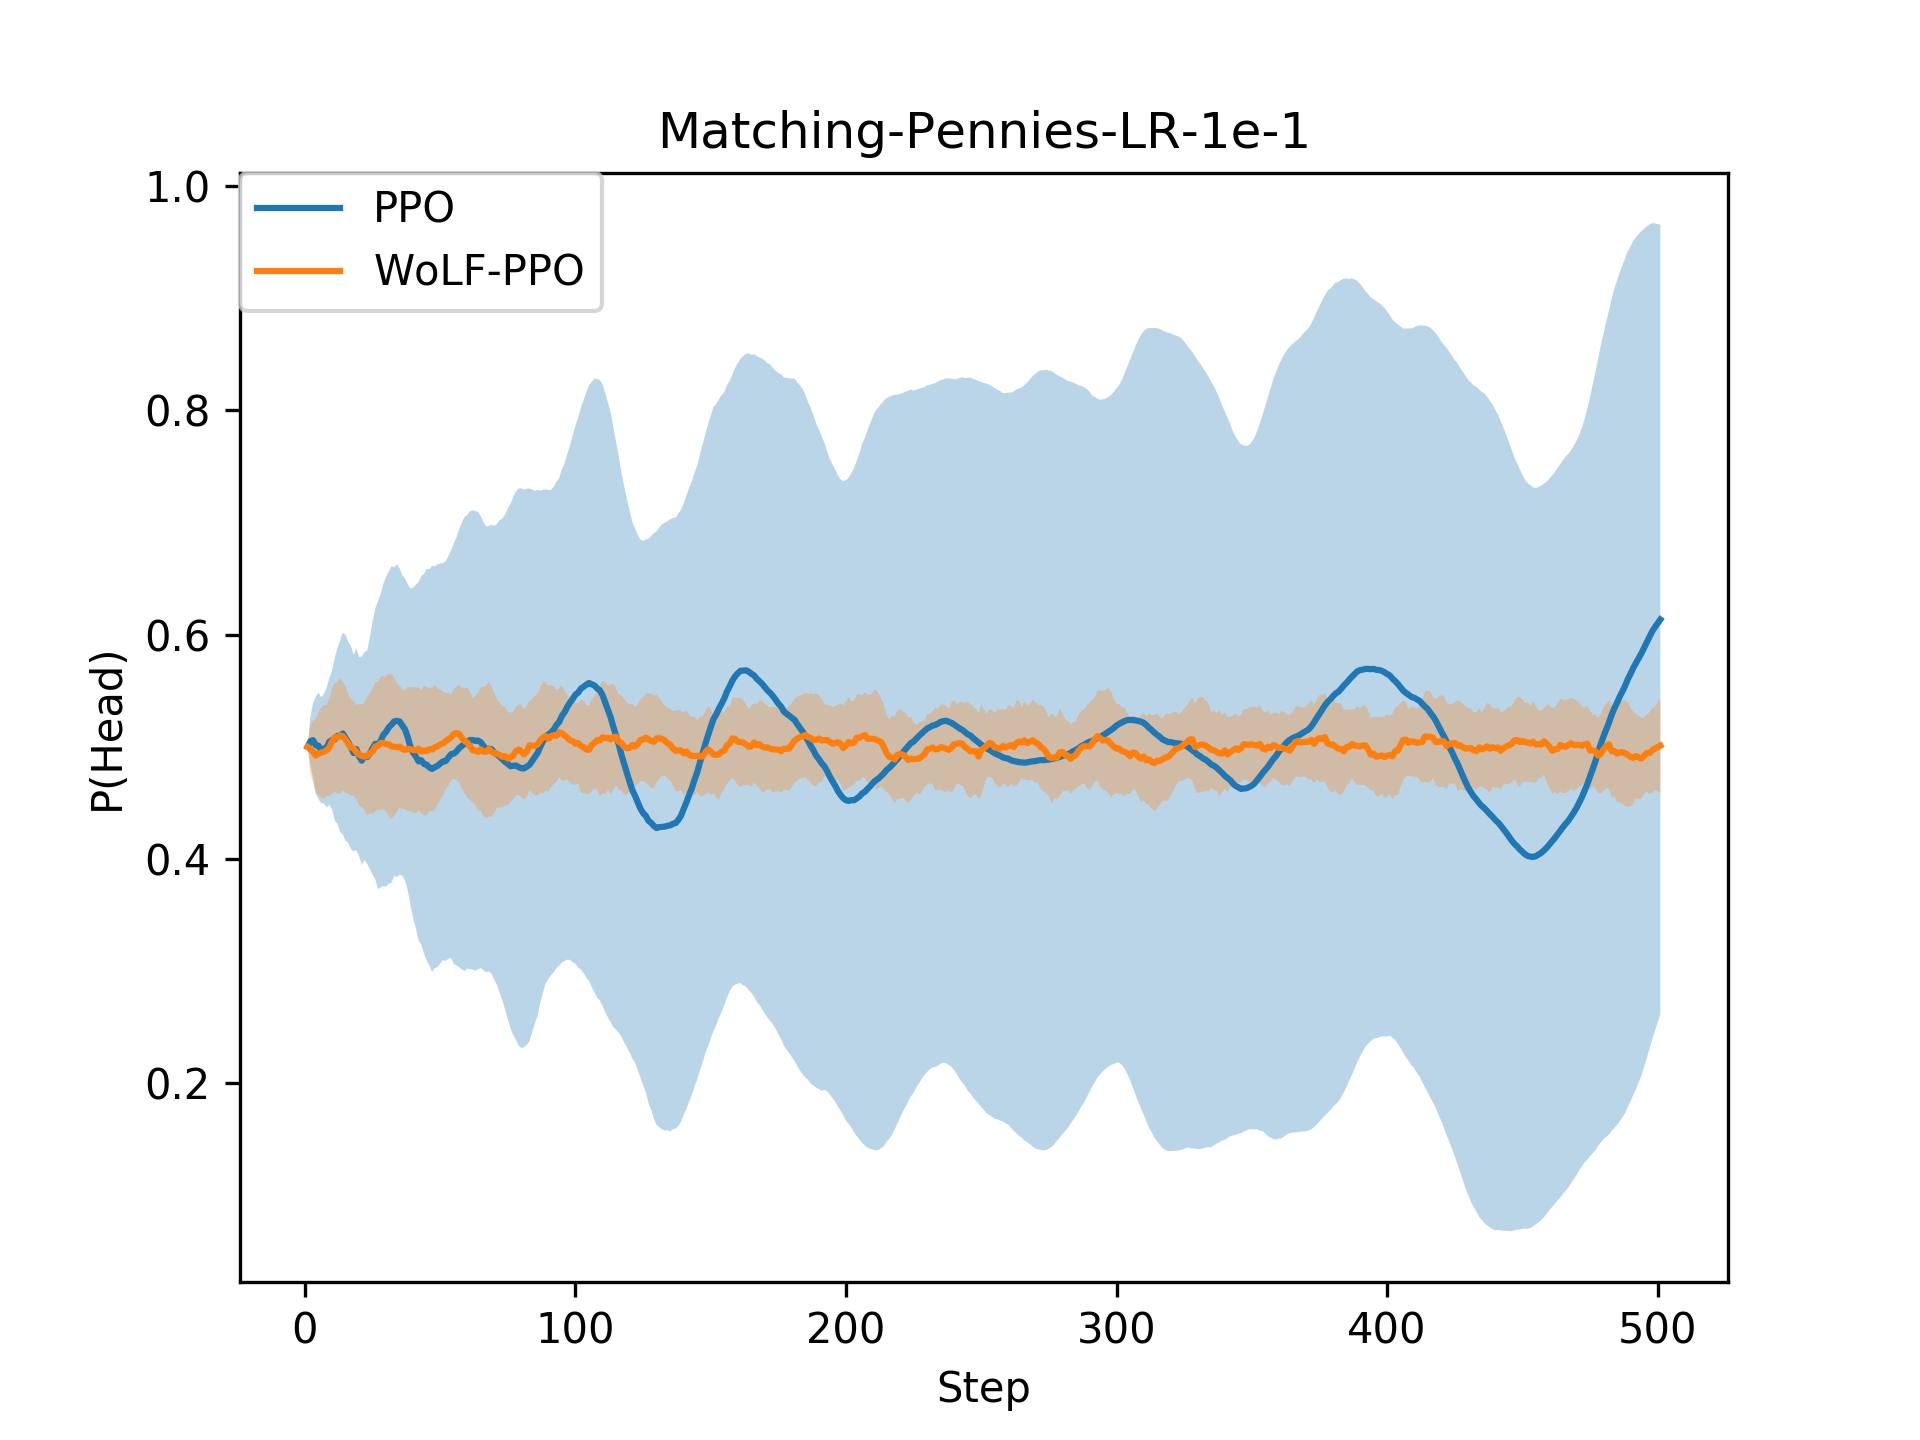
\includegraphics[width=20em]{Figures/matching-pennies-lr-1e-1.png}
    \caption{With a learning rate an order of magnitude higher we begin to see a larger negative effect for PPO than that WoLF-PPO variant.}
    \label{fig:mp-ppo-e1}
\end{figure}

We demonstrate this phenomenon by using the weighted variant of Matching Pennies to push the Nash Equilibrium away from the max entorpy policy. In Fig \ref{fig:weighted-mp-ppo-e2} we can see that PPO now wildly diverges away from the Nash equilibrium strategy, with the variance being larger than when dealing with the non weighted matching pennies. We also see that WoLF-PPO outperforms PPO by a larger amount in this environment, showing the benefit of WoLF-PPO in environments without the Nash equilibrium lying on the max entropy strategy.

\begin{figure}
    \centering
    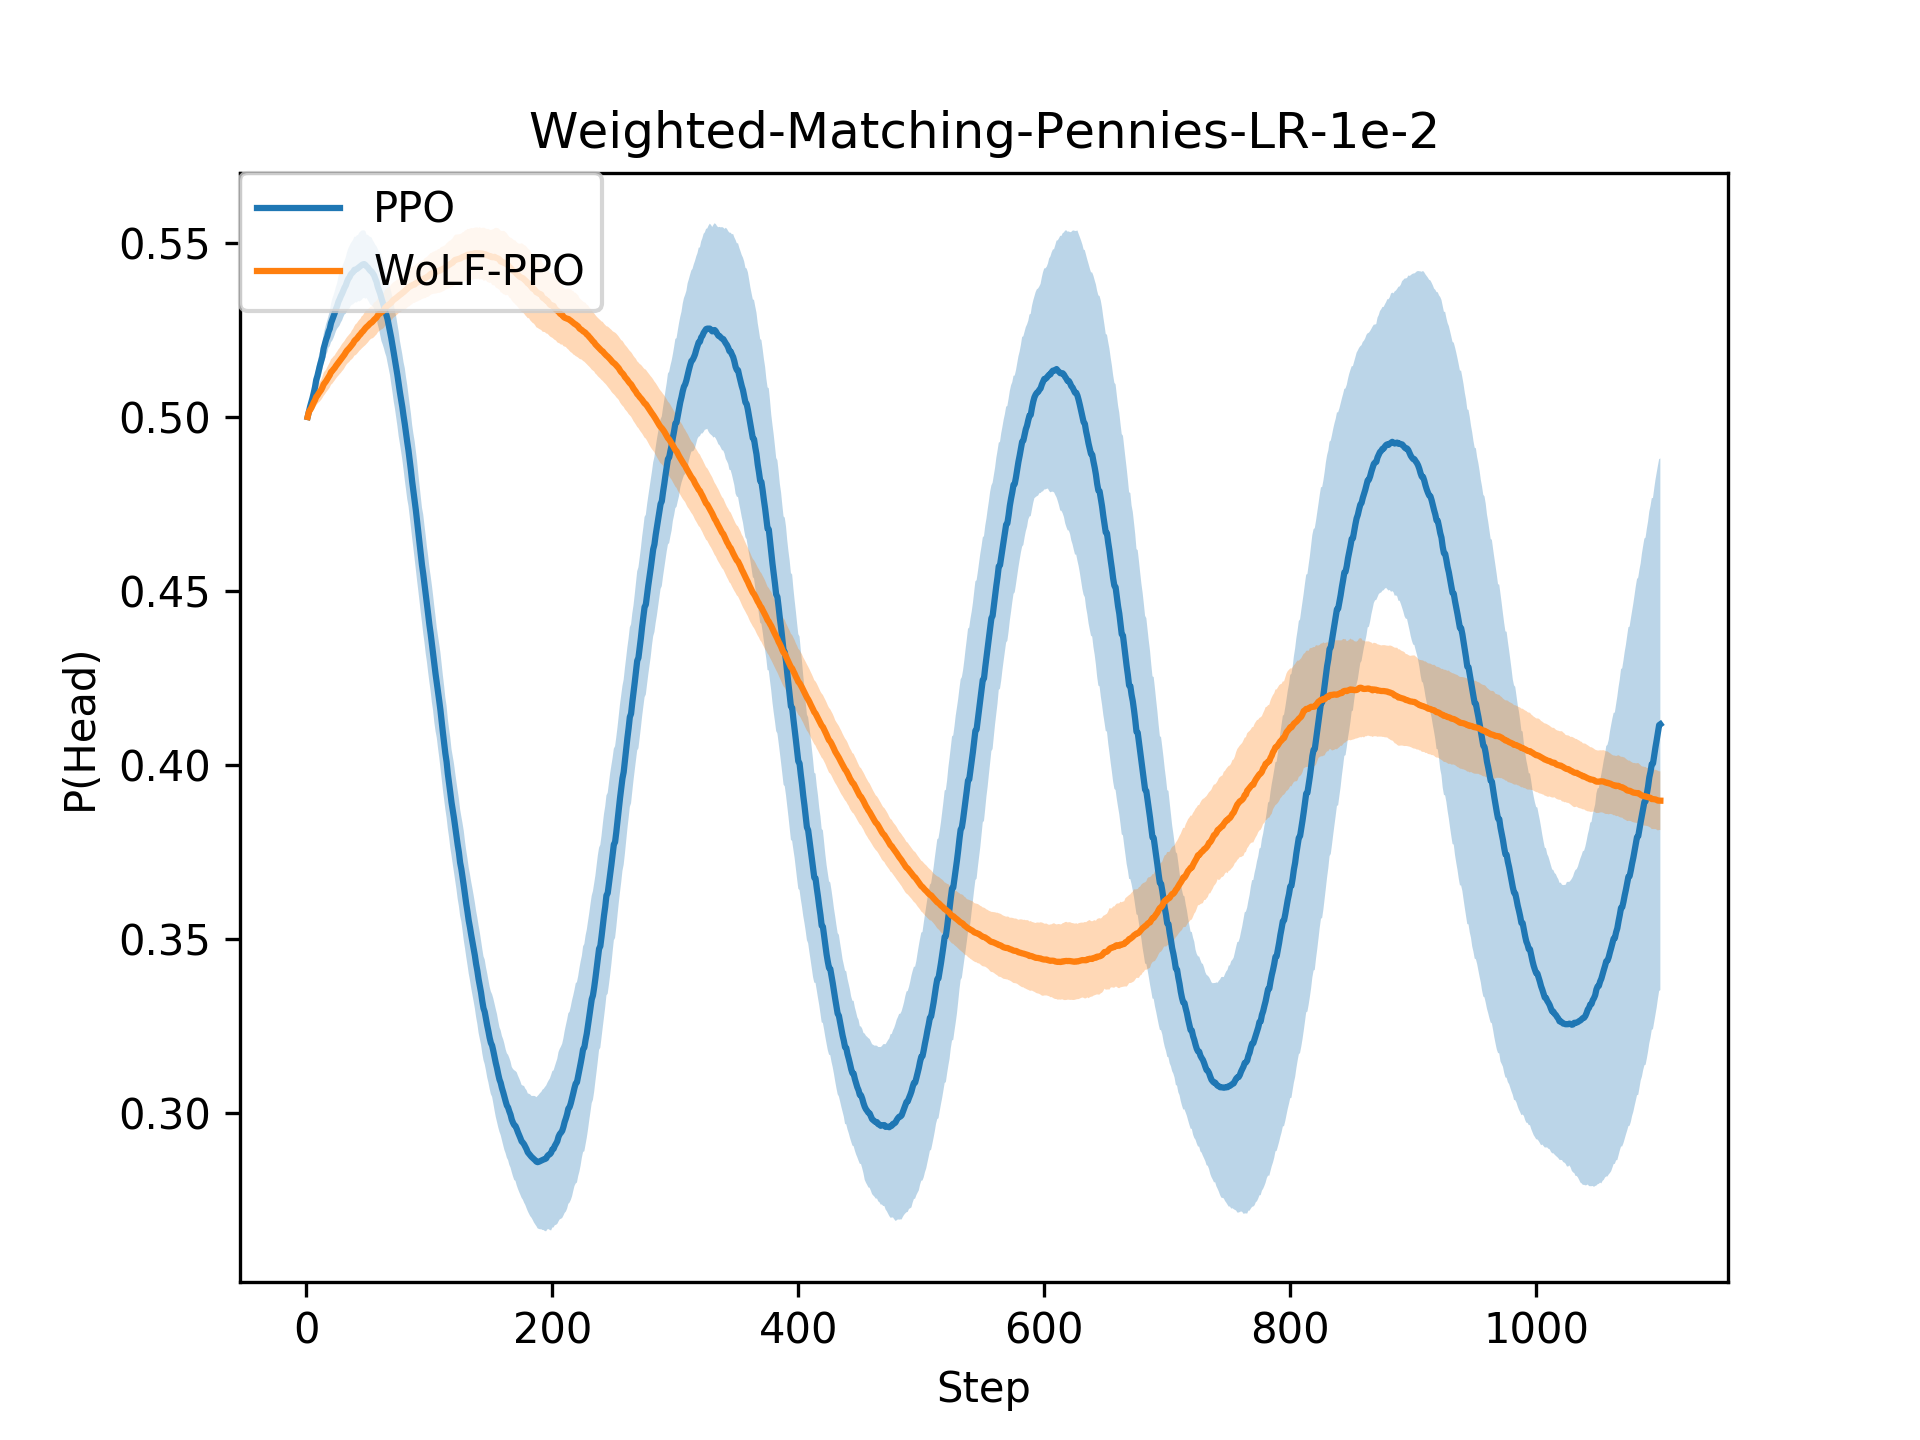
\includegraphics[width=20em]{Figures/weighted-matching-pennies-lr-1e-2.png}
    \caption{With a reasonable learning rate of 2.5e-4 on the weighted variant of matching pennies we see that WoLF-PPO now greatly out performs PPO.}
    \label{fig:weighted-mp-ppo-e2}
\end{figure}

\subsection{Rock Paper Scissors}

In Rock Paper Scissors we see very similar results to what we observed in matching pennies. In Fig \ref{fig:rps-ppo-e2} we show a sample run of PPO and WoLF-PPO, as shown they both stay close to the Nash equilibrium, as with standard matching pennies the Nash equilibrium lays on the max entropy strategy resulting in relatively good performance from PPO. When increasing the learning rate by an order of magnitude we end up with WoLF-PPO showing reduced variance, shown in Fig \ref{fig:rps-ppo-e1}. This is the same behaviour observed in matching pennies.

\begin{figure}
    \centering
    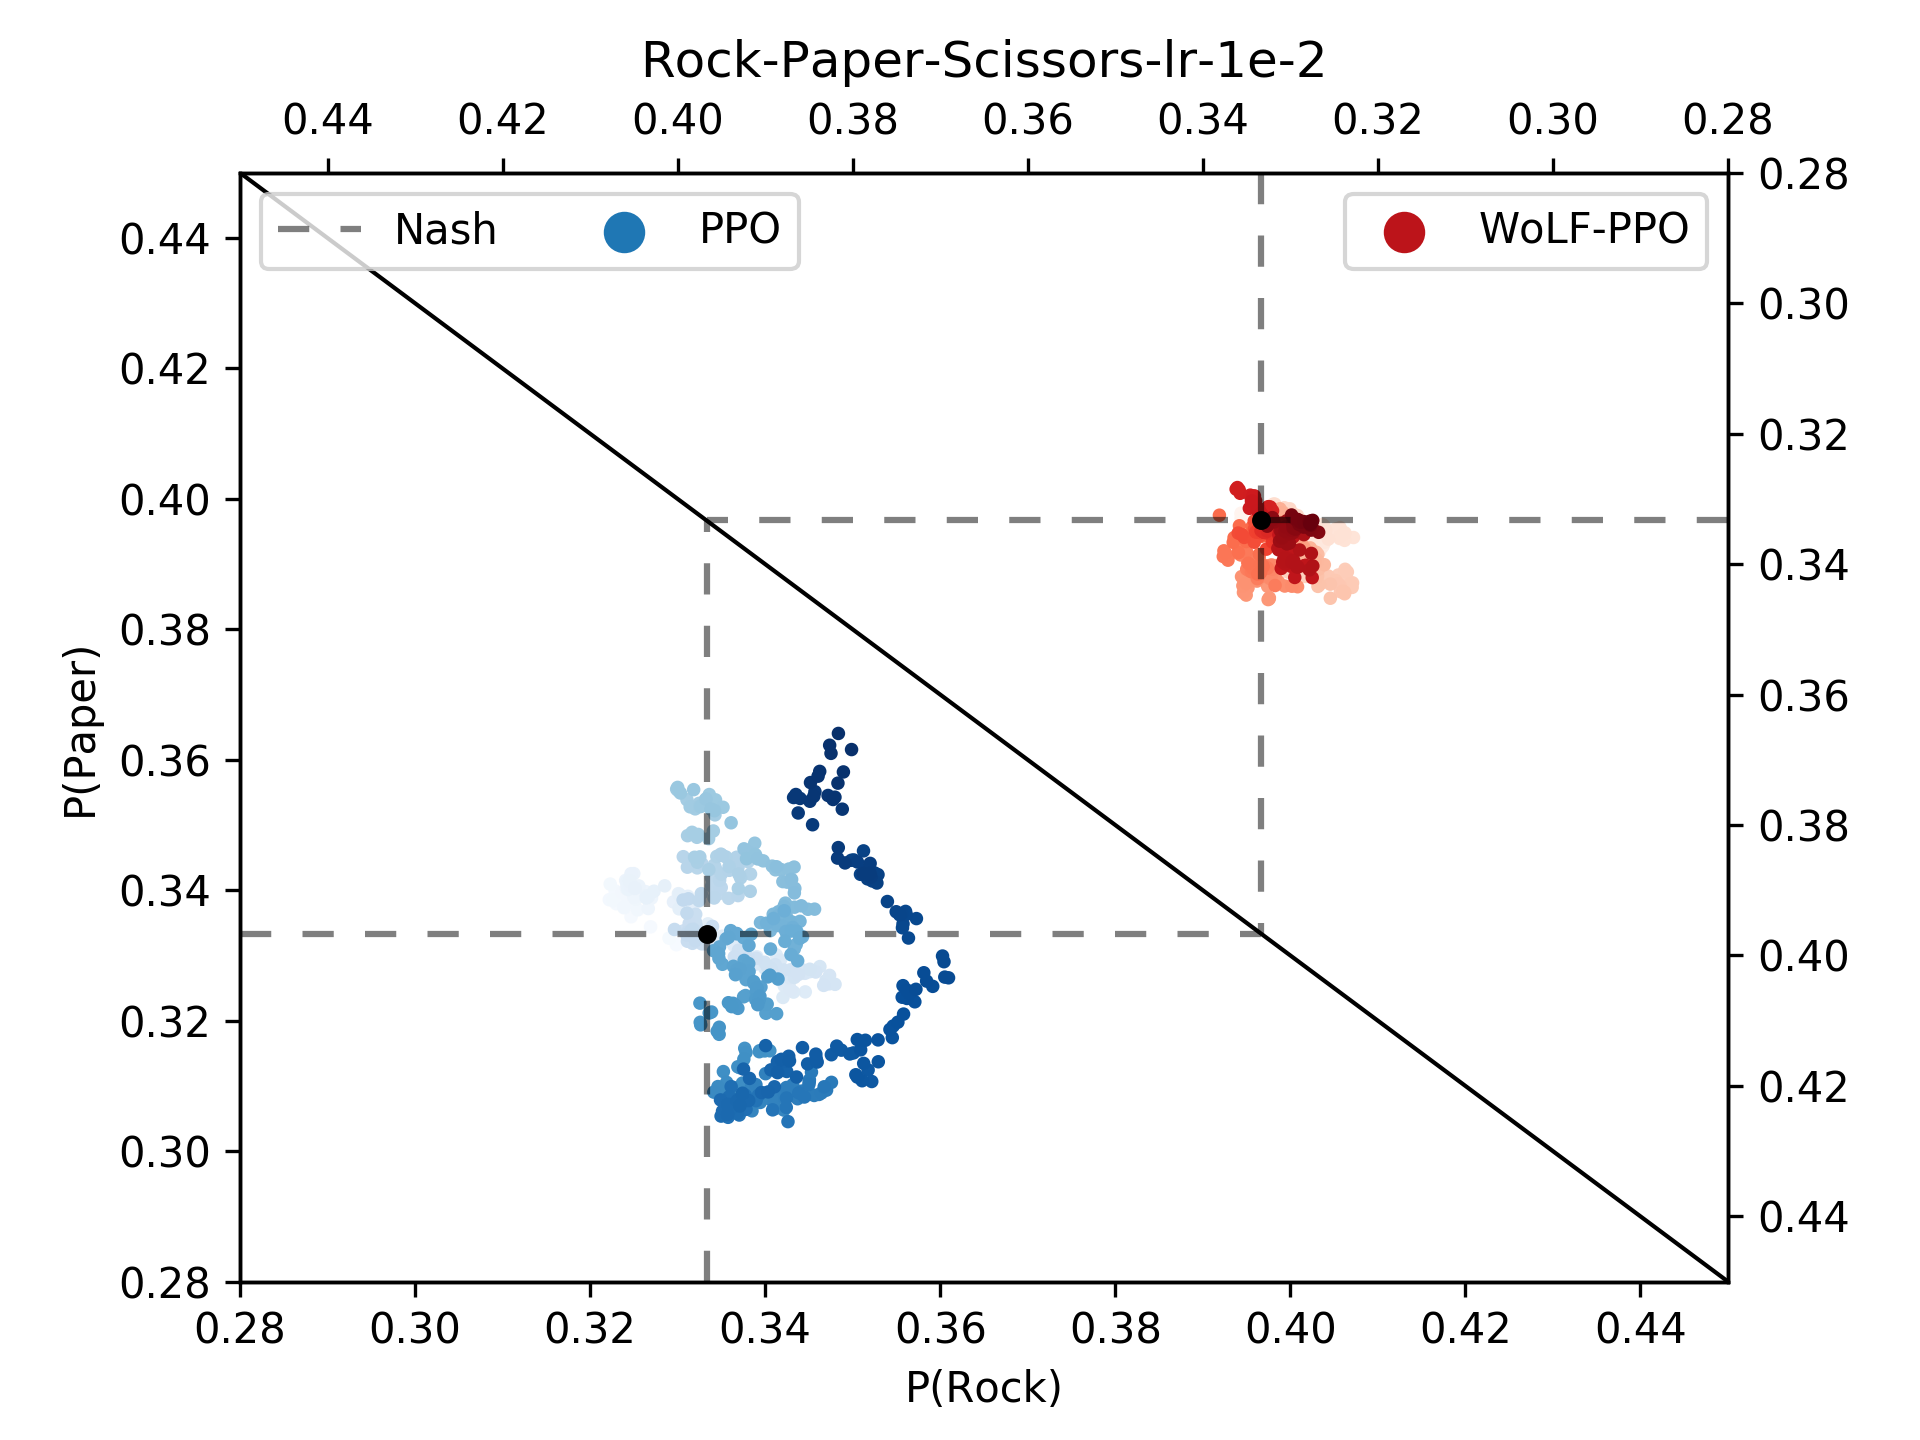
\includegraphics[width=20em]{Figures/rock-paper-scissors-lr-1e-2}
    \caption{Standard Rock Paper Scissors PPO and WoLF-PPO comparison}
    \label{fig:rps-ppo-e2}
\end{figure}

\begin{figure}
    \centering
    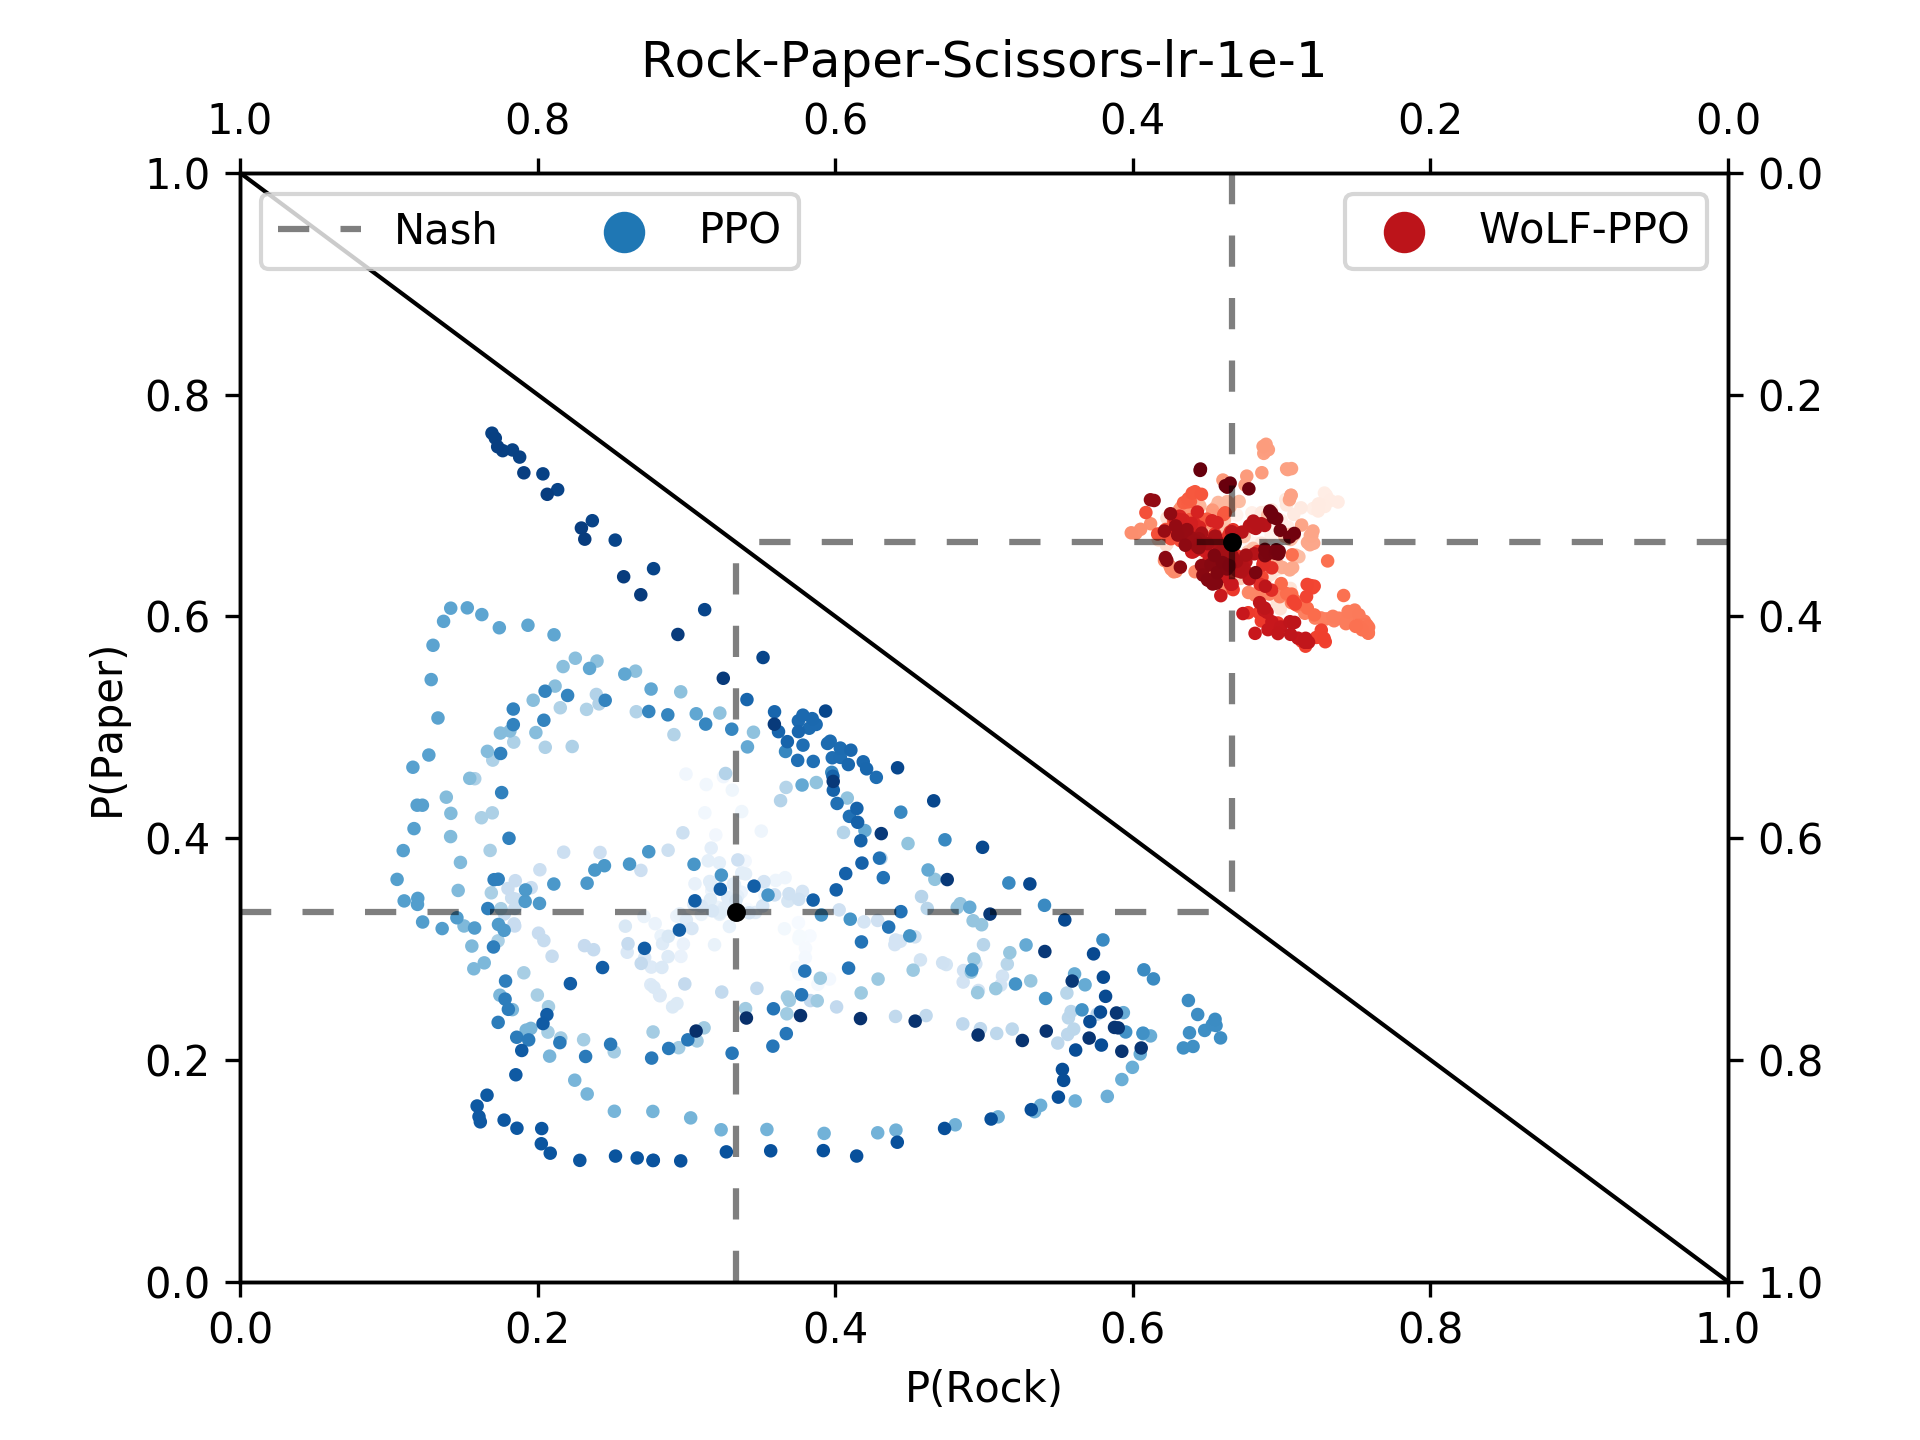
\includegraphics[width=20em]{Figures/rock-paper-scissors-lr-1e-1}
    \caption{Standard Rock Paper Scissors PPO and WoLF-PPO comparison, with a learning rate and order of magnitude higher}
    \label{fig:rps-ppo-e1}
\end{figure}

We then ran PPO and WoLF-PPO on a weighted version of Rock Paper Scissors. This is to move the Nash equilibrium away from the max entropy policy. In Fig \ref{fig:weighted-rps-ppo-e4} we show that in this environment WoLF-PPO stays closer to the Nash equilibrium than PPO. This is consistent with the matching pennies results. We also show in Fig \ref{fig:weighted-rps-ppo-e1} that even when increasing the learning rate by an order of magnitude WoLF-PPO is still able to outperform PPO, the distance from the Nash equilibrium is increased however not to the degree of PPO.

\begin{figure}
    \centering
    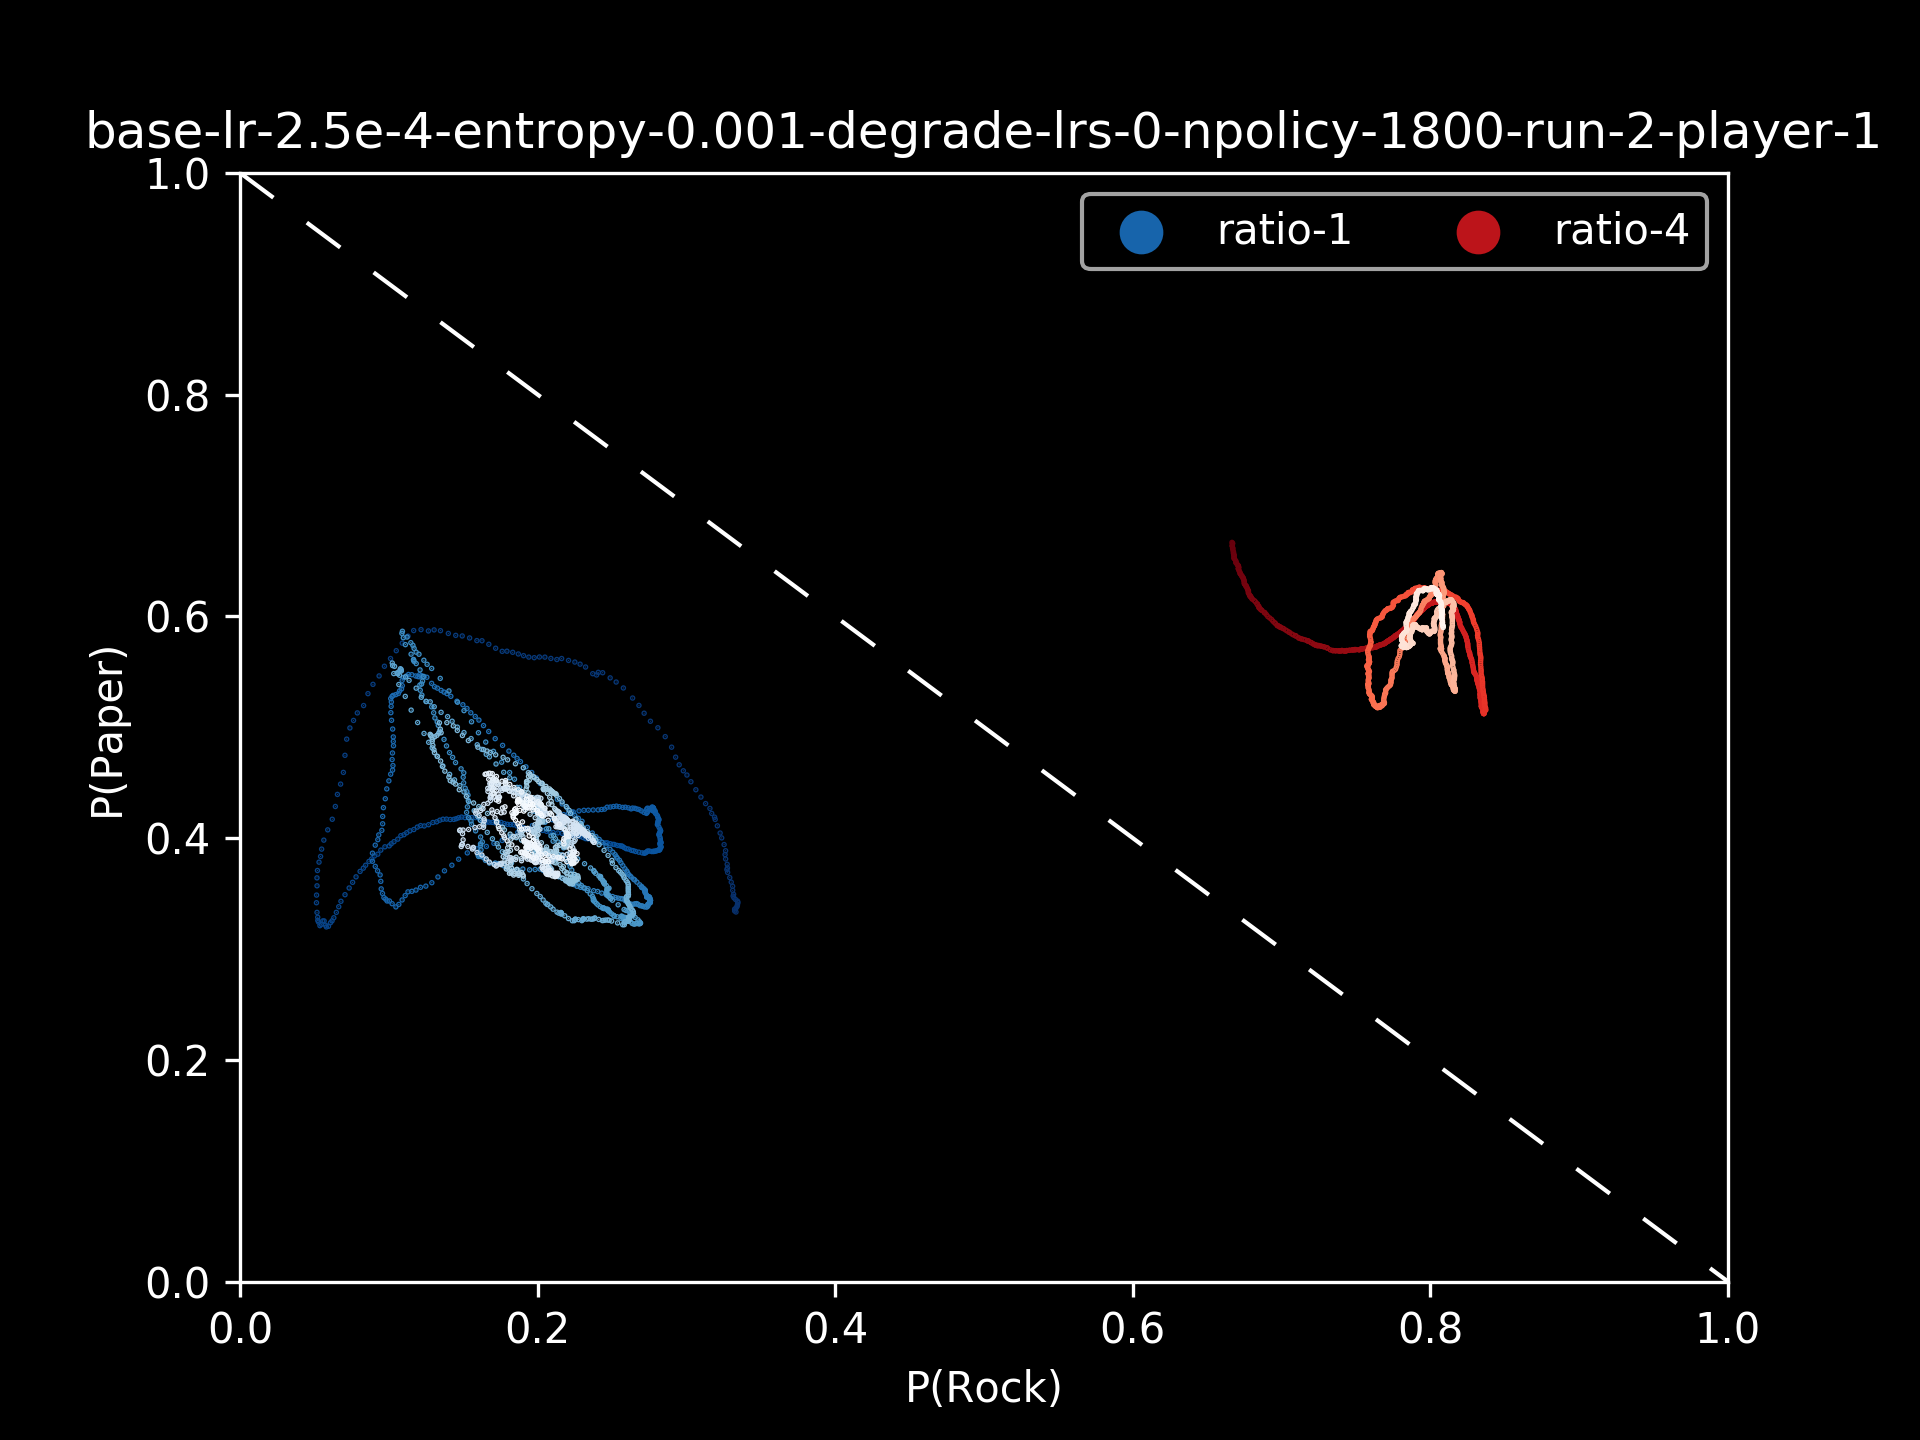
\includegraphics[width=20em]{Figures/weighted-rps-ppo-e4.png}
    \caption{Weighted Rock Paper Scissors PPO and WoLF-PPO comparison}
    \label{fig:weighted-rps-ppo-e4}
\end{figure}

\begin{figure}
    \centering
    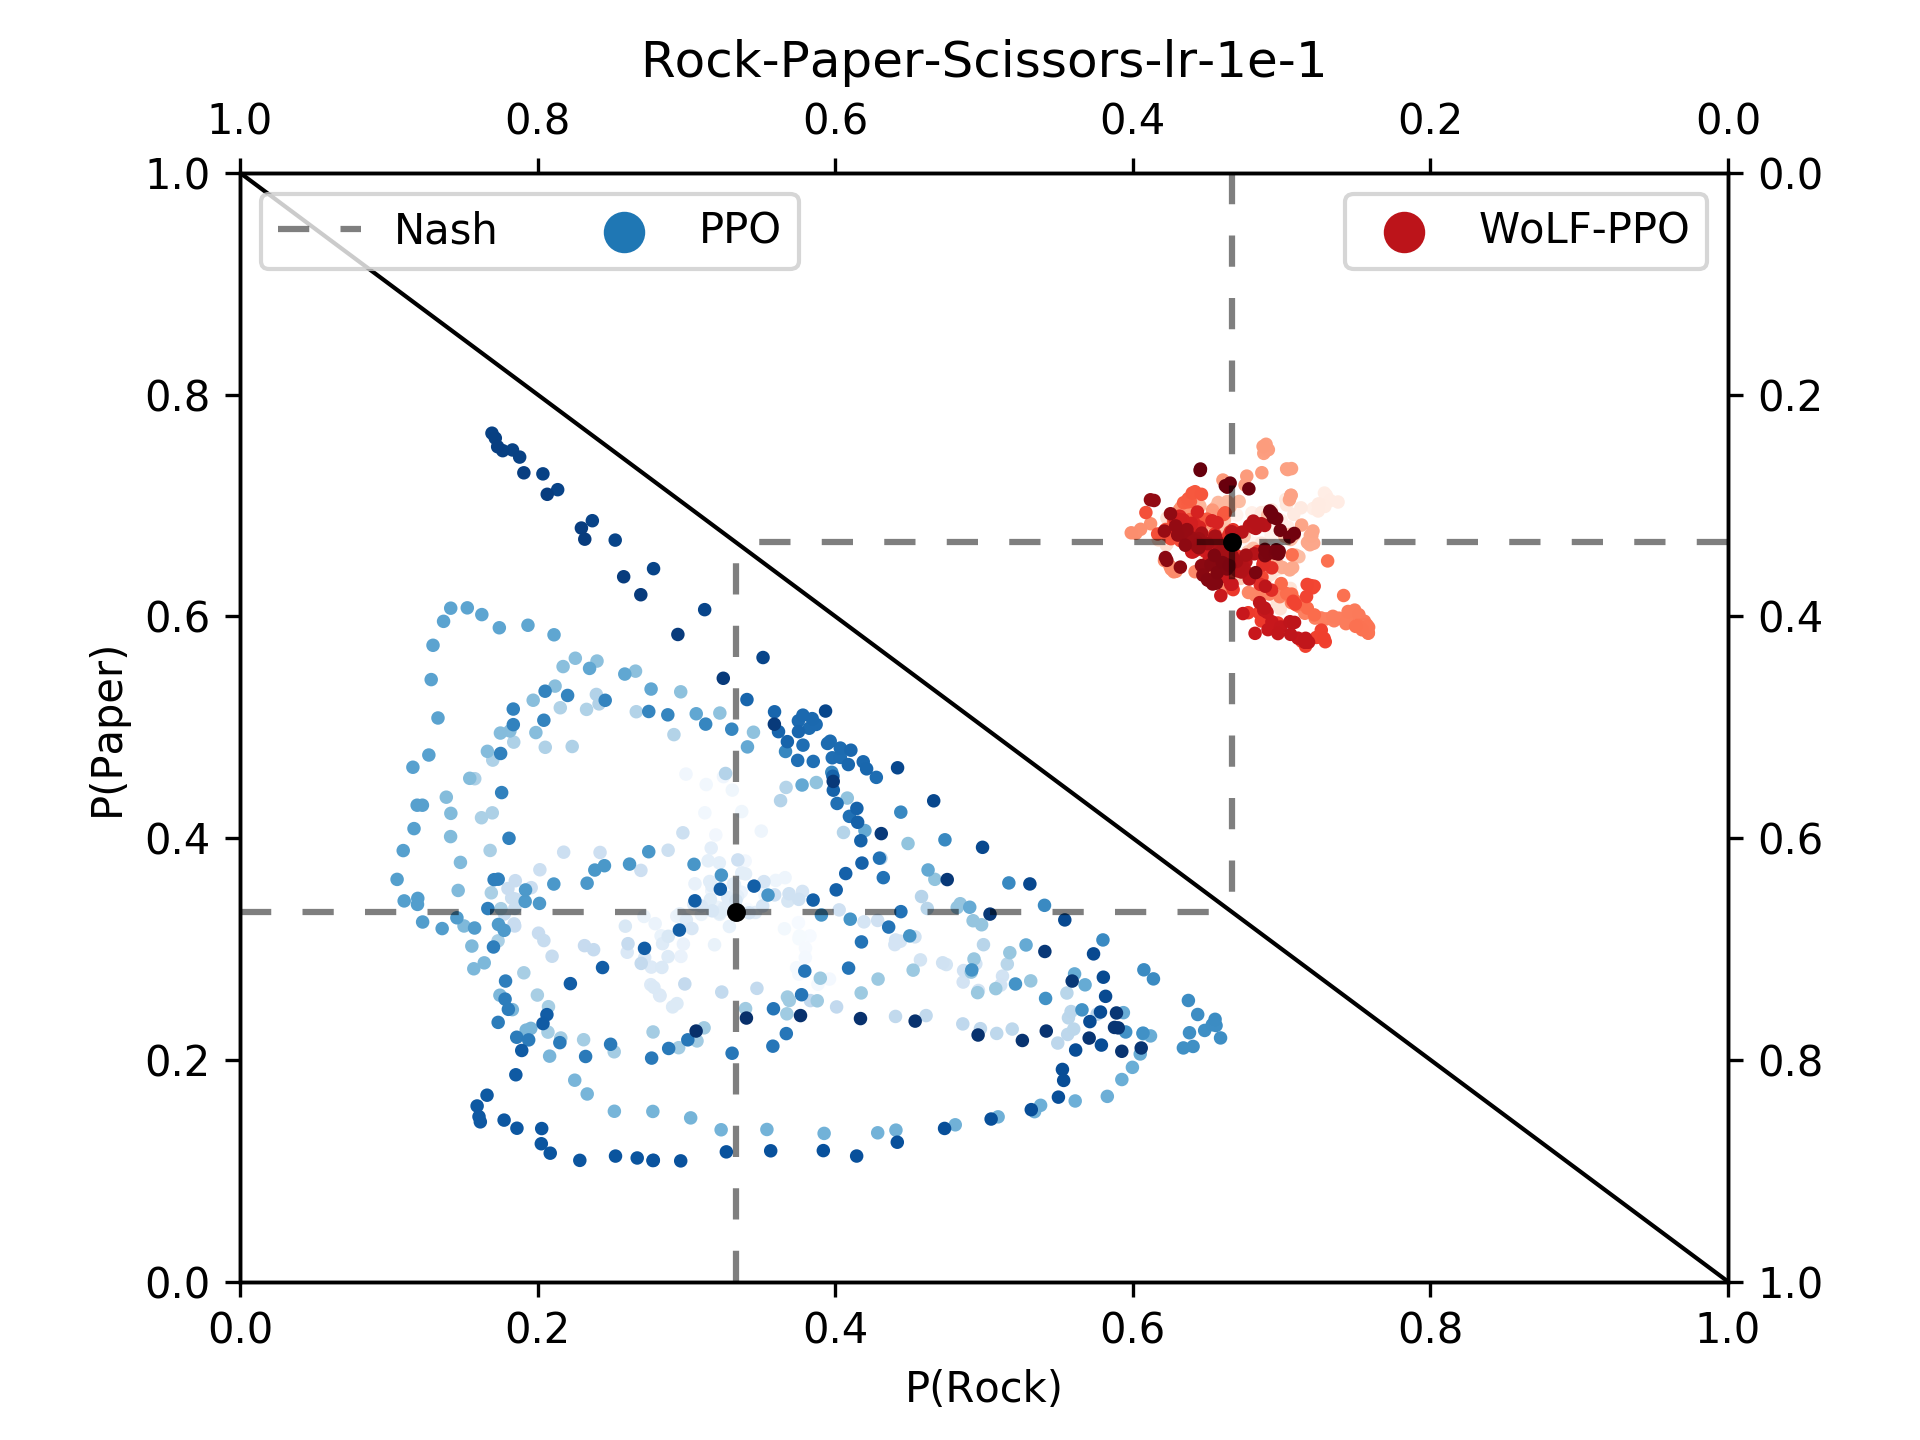
\includegraphics[width=20em]{Figures/rock-paper-scissors-lr-1e-1}
    \caption{Weighted Rock Paper Scissors PPO and WoLF-PPO comparison, with a learning rate and order of magnitude higher}
    \label{fig:weighted-rps-ppo-e1}
\end{figure}

\section{Conclusion}

% Connection with IPD - hysteretic agents ... questions around assessing "winning" or "losing" in more general games

In this paper we wanted to investigate if WoLF can be extended to Deep Reinforcment learning. We did this by comparing PPO to WoLF-PPO and evaluating the differences when learning the traditional game theory games Matching Pennies and Rock Paper Scissors. We also created variants of these games in order to shift the Nash off the max-entropy policy.

In our experiments we showed that the performance of PPO in both standard MP and RPS is better than originally expected. We believe this is due to the fact that the Nash equilibrium for these games lies on the max-entropy policy. PPO contains a max-entropy term in its objective function, this means that PPO has an unfair advantage in these specific environments due to the Nash equilibrium being directly optimised by the max-entropy term in the objective function. When training on variants of MP and RPS to shift the Nash Equilibrium off the max-entropy policy we observe that WoLF now provides a much greater advantage over traditional PPO as the agent now learns a policy much closer to the nash equilibrium. We also observed that WoLF-PPO is more robust than PPO when dealing with large learning rates.

In this work we have demonstrated that the WoLF approach can be extended to Deep RL while providing benefits when learning in multi-agent environments, getting closer to the nash equilibrium. We would like to expand this to extensive form games in the future, specifically the Soccer environment. We would then like to expand beyond what is possible with tabular RL in order to demonstrate both the advantages of WoLF and Deep RL by training on raw pixel data.

\end{document}
